%Version 2.1 April 2023
% See section 11 of the User Manual for version history
%
%%%%%%%%%%%%%%%%%%%%%%%%%%%%%%%%%%%%%%%%%%%%%%%%%%%%%%%%%%%%%%%%%%%%%%
%%                                                                 %%
%% Please do not use \input{...} to include other tex files.       %%
%% Submit your LaTeX manuscript as one .tex document.              %%
%%                                                                 %%
%% All additional figures and files should be attached             %%
%% separately and not embedded in the \TeX\ document itself.       %%
%%                                                                 %%
%%%%%%%%%%%%%%%%%%%%%%%%%%%%%%%%%%%%%%%%%%%%%%%%%%%%%%%%%%%%%%%%%%%%%

\documentclass[sn-vancouver,Numbered,lineno,pdflatex]{sn-jnl}

%%%% Standard Packages
%%<additional latex packages if required can be included here>

\usepackage{graphicx}%
\usepackage{multirow}%
\usepackage{amsmath,amssymb,amsfonts}%
\usepackage{amsthm}%
\usepackage{mathrsfs}%
\usepackage[title]{appendix}%
\usepackage{xcolor}%
\usepackage{textcomp}%
\usepackage{manyfoot}%
\usepackage{booktabs}%
\usepackage{algorithm}%
\usepackage{algorithmicx}%
\usepackage{algpseudocode}%
\usepackage{listings}%
%%%%

%%%%%=============================================================================%%%%
%%%%  Remarks: This template is provided to aid authors with the preparation
%%%%  of original research articles intended for submission to journals published
%%%%  by Springer Nature. The guidance has been prepared in partnership with
%%%%  production teams to conform to Springer Nature technical requirements.
%%%%  Editorial and presentation requirements differ among journal portfolios and
%%%%  research disciplines. You may find sections in this template are irrelevant
%%%%  to your work and are empowered to omit any such section if allowed by the
%%%%  journal you intend to submit to. The submission guidelines and policies
%%%%  of the journal take precedence. A detailed User Manual is available in the
%%%%  template package for technical guidance.
%%%%%=============================================================================%%%%

\usepackage{natbib}
\usepackage{hyperref}
\usepackage[utf8]{inputenc}
\usepackage{capt-of}
\usepackage{booktabs}
\usepackage{amssymb}
\usepackage{threeparttable}
\usepackage{float}
%\floatplacement{figure}{H}
%\floatplacement{table}{H}
\usepackage{lipsum,caption}
\geometry{
  a4paper,
  left=1in,
  right=1in,
  top=1in,
  bottom=1in,
  includeheadfoot
}
\usepackage{setspace}
%\usepackage{lineno}
%\linenumbers
\usepackage{siunitx}
\sisetup{
  mode = match,
  propagate-math-font = true,
  reset-math-version = false,
  reset-text-family = false,
  reset-text-series = false,
  reset-text-shape = false,
  text-family-to-math = true,
  text-series-to-math = true
}
\doublespacing
% Disable explicit page breaks in LaTeX
\let\clearpage\relax



\raggedbottom




% tightlist command for lists without linebreak
\providecommand{\tightlist}{%
  \setlength{\itemsep}{0pt}\setlength{\parskip}{0pt}}





\begin{document}


\title[High-Dimensional Propensity Score]{Understanding the role of
different proxy selection methods in High-Dimensional Propensity Score
Framework - A Plasmode simulation study}

%%=============================================================%%
%% Prefix	-> \pfx{Dr}
%% GivenName	-> \fnm{Joergen W.}
%% Particle	-> \spfx{van der} -> surname prefix
%% FamilyName	-> \sur{Ploeg}
%% Suffix	-> \sfx{IV}
%% NatureName	-> \tanm{Poet Laureate} -> Title after name
%% Degrees	-> \dgr{MSc, PhD}
%% \author*[1,2]{\pfx{Dr} \fnm{Joergen W.} \spfx{van der} \sur{Ploeg} \sfx{IV} \tanm{Poet Laureate}
%%                 \dgr{MSc, PhD}}\email{iauthor@gmail.com}
%%=============================================================%%

\author*[1,2]{\pfx{Dr.} \fnm{Mohammad Ehsanul} \sur{Karim} \dgr{MSc,
PhD}}\email{\href{mailto:ehsan.karim@ubc.ca}{\nolinkurl{ehsan.karim@ubc.ca}}}

\author[3]{\fnm{Yang} \sur{Lei} }



  \affil*[1]{\orgdiv{School of Population and Public
Health}, \orgname{University of British
Columbia}, \orgaddress{\city{Vancouver}, \country{Canada}, \postcode{V6T
1Z3}, \state{BC}, \street{2206 East Mall}}}
  \affil[2]{\orgname{St.~Paul's
Hospital}, \orgaddress{\city{Vancouver}, \country{Canada}, \postcode{V6Z
1Y6}, \state{BC}, \street{588 - 1081 Burrard Street}}}
  \affil[3]{\orgdiv{Department of Statistics}, \orgname{University of
British
Columbia}, \orgaddress{\city{Vancouver}, \country{Canada}, \postcode{V6T
1Z4}, \state{BC}, \street{Room 3182 Earth Sciences Building, 2207 Main
Mall}}}

\abstract{\textbf{Purpose}: We aims to evaluate various proxy selection
methods within the context of high-dimensional propensity score (hdPS)
analysis. The study focuses on assessing the performance of these
methods, including alternative variable selection approaches, in
selecting proxy variables for confounding adjustment compared to the
traditional hdPS method that is rooted in Bross formula. The goal is to
understand better the performance of these alternative methods in
estimating treatment effects, and identify scenarios in which they may
perform better. \textbf{Methods:} Using data from three cycles of the
National Health and Nutrition Examination Survey (NHANES) spanning
2013-2018, we motivated the study by examining the association between
obesity and diabetes. A plasmode simulation framework based on this data
was employed to mimic real-world data structures. Simulations were
conducted under three scenarios: Frequent Exposure and Outcome, Rare
Exposure and Frequent Outcome, and Frequent Exposure and Rare Outcome.
The performance of a variety of proxy selection methods---including
tree-based methods, LASSO-based methods, and the Genetic Algorithm
(GA)---was evaluated across these scenarios using standard simulation
metrics. \textbf{Results:} XGBoost consistently demonstrated the lowest
MSE and high coverage, making it a reliable method overall, although it
did not always exhibit the lowest bias. In contrast, GA consistently
showed the highest bias and MSE, with lower coverage and greater
variability, indicating its unsuitability for accurate effect
estimation. The kitchen sink model, Bross-based hdPS, and Hybrid hdPS
methods performed moderately well, with low bias and moderate MSE, but
varied in coverage across scenarios. Scenario-specific trends revealed
that rare outcome scenarios yielded lower MSE and better precision,
while rare exposure scenarios were associated with higher bias and MSE.
\textbf{Conclusion:} Aside from GA, the performance of most other
methods in your study appears to be comparable in each scenario, though
with some variations depending on specific metrics. The findings
underscore the importance of selecting appropriate methods for hdPS
analysis based on the characteristics of the data, particularly the
prevalence of exposure and outcome. While XGBoost excelled in overall
accuracy and precision, the choice of method should be tailored to the
specific epidemiological goal to optimize bias, coverage, and precision
in estimating treatment effects.}

\keywords{Machine learning, Propensity score, Deep learning, Causal
inference}


\pacs[JEL Classification]{C18}
\pacs[MSC Classification]{92D30, 62P10}

\maketitle

\section{Background}\label{background}

\textcolor{red}{*need to write what hdps is, and why alternatives are considered*}

\textbf{Aim}: The aim of this research is to systematically evaluate and
compare different proxy selection methods within the context of
high-dimensional propensity score (hdPS) analysis. Specifically, the
study focuses on assessing how these methods, including alternative
variable selection approaches, perform in selecting proxy variables for
confounding adjustment compared to the traditional Bross method within
the hdPS framework. We seek to determine whether these alternative
methods offer superior performance in estimating treatment effects
compared to the default Bross formula.

\section{Methods}\label{methods}

\subsection*{Data and Simulation}\label{data-and-simulation}
\addcontentsline{toc}{subsection}{Data and Simulation}

\textbf{Motivating Example}: To explore the relationship between obesity
and the risk of diabetes, we revisited this association using data from
three cycles of the National Health and Nutrition Examination Survey
(NHANES) covering the years 2013-2014, 2015-2016, and 2017-2018
\citep{karim2024high}. This analysis was informed by a thorough review
of the existing literature
\citep{saydah2014trends, liu2013association, kabadi2012joint, ostchega2012abdominal}.
To identify relevant covariates, we constructed a causal diagram based
on established causal inference principles \citep{greenland1999causal}.
The covariates included in our analysis were carefully selected and
categorized into Demographic, Behavioral, Health History,
Access-related, and Laboratory variables \citep{karim2024high}. While
most of these variables were binary or categorical, the Laboratory
variables were continuous.

\textbf{Plasmode simulation}: To rigorously assess the performance of
the methods under consideration, we employed a plasmode simulation
framework, which is particularly well-suited for reflecting real-world
data structures and complexities \citep{franklin2014plasmode}. This
approach was modeled after the analytic dataset derived from NHANES and
involved resampling from the observed covariates and exposure
information (i.e., obesity) without altering them. By mirroring key
aspects of an actual epidemiological study, this simulation framework
offers a significant advantage over traditional Monte Carlo simulations,
which often rely on idealized assumptions.

\textbf{Simulation scenarios under consideration}: Our plasmode
simulation was conducted over 500 iterations. For the base simulation
scenario, we set the prevalence of exposure (obesity) and the event rate
(diabetes) at 30\%, with a true odds ratio (OR) parameter of 1,
corresponding to a risk difference (RD) of 0. Each simulated dataset had
a sample size of 3,000 participants. The description of other scenarios
under consideration is provided in Table \ref{table:scenarios}.

\begin{table}[ht]
\centering
\caption{Overview of Plasmode Simulation Scenarios Reflecting Varying Exposure and Outcome Prevalences Based on National Health and Nutrition Examination Survey (NHANES) Data Cycles (2013-2018)}
\label{table:scenarios}
\begin{tabular}{lcccc}
  \toprule
  \textbf{Plasmode Simulation Scenario} & \textbf{Exposure} & \textbf{Outcome} & \textbf{True} & \textbf{Sample}\\
  \textbf{} & \textbf{Prevalence} & \textbf{Prevalence} & \textbf{Odds Ratio} & \textbf{Size}\\
  \midrule
  (i) Frequent Exposure and Outcome (Base) & 30\% & 30\% & 1 & 3,000 \\
  (ii) Rare Exposure and Frequent Outcome & 5\% & 30\% & 1 & 3,000 \\
  (iii) Frequent Exposure and Rare Outcome & 30\% & 5\% & 1 & 3,000 \\
  \bottomrule
\end{tabular}
\end{table}

\textbf{True Data Generating Mechanism Used in Plasmode Simulation}: The
primary goal of this study is to evaluate various variable selection
methods under realistic conditions. To achieve this, we formulated the
outcome data based on a specific model specification that incorporates
both exposure and covariates, including investigator-specified and proxy
variables. The model specification consists of three key components (See
Appendices \S A and B for further details):

\begin{enumerate}
\def\labelenumi{\arabic{enumi}.}
\item
  \emph{Investigator-Specified Covariates}: We retained the original
  investigator-specified covariates, which were either binary or
  categorical, reflecting how real-world studies typically operate.
\item
  \emph{Transformation of Laboratory Variables}: In real-world studies,
  it is common for analysts to lack precise knowledge of the true model
  specification. To simulate this uncertainty, we transformed the
  continuous laboratory variables using complex functions such as
  logarithmic, exponential, square root, polynomial transformations, and
  interactions. This reflects the challenges analysts face in correctly
  specifying models when dealing with continuous data.
\item
  \emph{Inclusion of Proxy Variables}: Real-world studies often deal
  with unmeasured confounding, which researchers attempt to mitigate by
  adding proxy variables. However, when a large number of proxies are
  added, some may act as noise variables, contributing little to the
  analysis. To simulate this, we selected only those binary proxy
  covariates (referred to as recurrence covariates in hdPS terminology)
  that had a relative risk (RR) of less than 0.8 or greater than 1.2
  concerning the outcome. Out of 143 proxy covariates, 94 met this
  criterion and were included in calculating a simple comorbidity burden
  measure. The remaining 49 covariates were excluded from this
  calculation and considered noise. This comorbidity burden measure was
  then incorporated into our model specification for generating the
  plasmode data.
\end{enumerate}

\textbf{Performance Measures}: From this simulation, we derived several
performance metrics to evaluate the effectiveness of the methods under
consideration: (1) bias, (2) average model standard error (SE; the
average of estimated SEs obtained from a model over repeated samples),
(3) empirical SE (the standard deviation of estimated treatment effects
across repeated samples), (4) mean squared error (MSE), (5) coverage
probability of 95\% confidence intervals, (6) bias-corrected coverage,
and (7) Zip plot \citep{morris2019using, white2023check}.

\subsection*{Estimators under
consideration}\label{estimators-under-consideration}
\addcontentsline{toc}{subsection}{Estimators under consideration}

\textcolor{red}{*check if the description of the methods look okay to you. Make sure the description matches with the analysis codes.*}

The comparison between the data generation process and the analysis
process reveals two key differences: (i) The data generation used
transformed laboratory variables, whereas the analysis was conducted
using only the original laboratory variables. (ii) The data generation
employed a simple sum of selected proxy variables (sum of 94 proxy
covariates), while the analysis included all proxy variables (143 binary
proxies), with 49 of these acting as noise variables. These differences
help us assess how the proxy variable selection methods handle model
misspecification and the presence of noise variables.

\begin{enumerate}
\def\labelenumi{\arabic{enumi}.}
\item
  \textbf{Kitchen sink model}: This is a base model for comparison,
  where no variable selection approaches were used. All
  investigator-selected features and all proxy variables were used to
  model \citep{karim2018can}.
\item
  \textbf{Bross formula}: The Bross formula is a statistical method used
  to calculate the bias introduced by not adjusting for a covariate
  \citep{bross1966spurious}. In hdPS analysis, this formula was
  originally applied to each proxy variable to measure and rank the
  potential bias if the covariate were not adjusted for. In our
  analysis, the 100 proxies with the highest bias rankings are selected
  for further modeling \citep{schneeweiss2009high, wyss2018erratum}.
\item
  \textbf{Least Absolute Shrinkage and Selection Operator (LASSO)}:
  LASSO is a variable selection technique that limits the number of
  variables by adding a penalty term to the regression model.
  Cross-validation (CV) is used in LASSO to identify variables with
  non-zero coefficients in the best model by optimizing the penalty
  value
  \citep{franklin2015regularized, schneeweiss2017variable, karim2018can}.
\item
  \textbf{Hybrid of hdPS and LASSO}: Instead of relying solely on LASSO
  for variable selection, a hybrid approach combines the Bross formula
  and LASSO. First, hdPS variables are selected using the hdPS algorithm
  (e.g., the top 100), and then LASSO is applied to further refine the
  selection \citep{karim2018can, franklin2015regularized}.
\item
  \textbf{Elasticnet}: Elastic Net is an extension of LASSO that
  includes an additional penalty term to handle multicollinearity by
  grouping correlated features and selecting the most representative
  ones \citep{karim2018can}.
\item
  \textbf{Random Forest}: The Random Forest (RF) algorithm is an
  ensemble learning method that constructs multiple decision trees to
  perform classification \citep{breiman2001random}. It calculates the
  importance of each proxy variable based on the decrease in impurity or
  Gini importance, providing a ranking of the proxies. The top 100
  variables from this ranking are manually selected for further modeling
  \citep{schneeweiss2017variable}.
\item
  \textbf{XGBoost}: XGBoost is a gradient boosting algorithm used to
  optimize machine learning models \citep{chen2016xgboost}. It builds
  decision trees that make splits based on maximum impurity reduction,
  and it assigns an importance score to each proxy variable by
  calculating the mean decrease in impurity
  \citep{xiao2024interpretable}.
\item
  \textbf{Stepwise}: Stepwise selection is a progressive feature
  selection method that can proceed in two directions---forward or
  backward---based on the maximum adjusted R-squared. We have
  implemented two versions: (a) Forward selection (FS) starts with an
  initial model (e.g., including all investigator-selected features) and
  adds proxies to the model one at a time. (b) Backward elimination (BE)
  starts with a full model (e.g., all investigator-selected features and
  all proxy variables) and removes features one at a time based on their
  contribution to the model.
\item
  \textbf{Genetic algorithm (GA)}: GA is an evolutionary algorithm
  inspired by the theory of natural selection
  \citep{holland1975adaptation}. It operates by evolving offspring from
  a population of the fittest individuals over several generations,
  evaluating and selecting the best combination of features or variables
  that maximize prediction accuracy.
\end{enumerate}

\section{Results}\label{results}

\textcolor{red}{*Can you check the app in the doc folder of the repo, and compare of the results description look accurate to you?*}

The results for each method under the different scenarios are summarized
below. See Figures \ref{fig:bias-comparison} and
\ref{fig:Coverage-comparison} for an overview of the performance in
terms of bias and coverage, respectively.

\begin{enumerate}
\def\labelenumi{(\roman{enumi})}
\tightlist
\item
  \textbf{Frequent Exposure and Outcome (base) scenario}:
\end{enumerate}

\begin{enumerate}
\def\labelenumi{\arabic{enumi}.}
\item
  \emph{Bias}: The kitchen sink model, which includes all variables
  without selection, exhibited the smallest bias (0.0002). GA shows the
  highest bias (0.0287), indicating a substantial deviation from the
  true effect. Among the other methods, Bross-based hdPS (-0.0001),
  Hybrid hdPS (0.0016), and Elasticnet (0.0036) demonstrated low bias.
  XGBoost (0.0074) and Random Forest (RF) (0.0034) still had slightly
  higher bias.
\item
  \emph{Coverage}: The coverage for most methods was high, with Hybrid
  hdPS, Forward Selection, Backward Elimination, LASSO, and Elasticnet
  achieving values around 98\%, indicating well-calibrated confidence
  intervals. However, GA had significantly lower coverage (83.8\%),
  indicating that its confidence intervals might be too narrow or
  biased, potentially missing the true effect. After applying bias
  elimination, GA's coverage improved to 96\%, which is better but still
  lower than other methods.
\item
  \emph{Mean Squared Error (MSE)}: XGBoost achieved the lowest MSE
  (0.0006), reaffirming it as the most accurate method overall. GA
  maintained the highest MSE (0.0016), reflecting its higher bias and
  variability. The kitchen sink model (0.0009), Bross-based hdPS
  (0.0008), Hybrid hdPS (0.0008), and Elasticnet (0.0009) all had
  relatively similar and moderate MSE values.
\item
  \emph{Standard Error (SE)}: XGBoost exhibited the lowest Empirical SE
  (0.0229), indicating high precision in its estimates. The kitchen sink
  model had the highest Empirical SE (0.0305), suggesting greater
  variability. Other methods, including GA (0.0274), Hybrid hdPS
  (0.0278), and Bross-based hdPS (0.0287), showed moderate variability.
  LASSO (0.0299) and Elasticnet (0.0294) had slightly higher
  variability. The Model-based SE followed a similar pattern, with
  XGBoost (0.0268) showing the lowest variability and the kitchen sink
  model (0.0333) the highest, indicating less precision in its
  estimates. See Appendix \S C for further details.
\end{enumerate}

\textbf{(ii) Rare Exposure and Frequent Outcome}:

\begin{enumerate}
\def\labelenumi{\arabic{enumi}.}
\item
  \emph{Bias}: The kitchen sink model showed a relatively low bias
  (0.0025), while GA continued to exhibit the highest bias (0.0408),
  indicating a significant deviation from the true effect. XGBoost had a
  bias of 0.0259, which, while still higher than some other methods, was
  lower than GA. Other methods, such as Bross-based hdPS (0.0035),
  Hybrid hdPS (0.0049), and Elasticnet (0.0053), demonstrated moderate
  bias. Random Forest (RF) (0.0127) and Forward Selection (0.0108) had
  slightly higher bias but remained within an acceptable range.
\item
  \emph{Coverage}: Coverage levels remained high for most methods, with
  XGBoost achieving the highest coverage at 96.2\%, indicating
  well-calibrated confidence intervals despite its higher bias. The GA
  method had lower coverage (92.2\%), suggesting that its confidence
  intervals might be narrower, potentially missing the true effect.
  Other methods such as RF, Forward Selection, Backward Elimination, and
  Hybrid hdPS maintained coverage values around 94-95\%, suggesting
  adequate interval calibration. Bias-eliminated coverage for GA
  improved to 94.2\%, but it was still slightly lower than other
  methods.
\item
  \emph{Mean Squared Error (MSE)}: Hybrid hdPS and XGBoost both
  demonstrated the lowest MSE (0.0032), indicating that these methods
  were the most accurate in this scenario. The GA method had a higher
  MSE (0.0043), reflecting its substantial bias and variability. The
  kitchen sink model also had an MSE of 0.0043, similar to GA, while
  other methods like Bross-based hdPS (0.0035), RF (0.0039), and
  Elasticnet (0.0036) exhibited moderate MSE values, indicating
  reasonable accuracy.
\item
  \emph{Standard Error (SE)}: The lowest Empirical SE was observed with
  XGBoost (0.0507) and GA (0.0510), reflecting high precision despite
  their higher bias. The kitchen sink model had the highest Empirical SE
  (0.0656), indicating greater variability. Hybrid hdPS (0.0564),
  Bross-based hdPS (0.0595), and RF (0.0609) showed moderate
  variability. Forward Selection (0.0537) and Backward Elimination
  (0.0576) had lower variability compared to the kitchen sink model. In
  terms of Model-based SE, XGBoost (0.0531) and GA (0.0533) continued to
  show low variability, while the kitchen sink model had the highest
  Model-based SE (0.0623), indicating less precision in its estimates.
\end{enumerate}

\textbf{(iii) Frequent Exposure and Rare Outcome}:

\begin{enumerate}
\def\labelenumi{\arabic{enumi}.}
\item
  \emph{Bias}: In this scenario, the kitchen sink model exhibited a
  moderate negative bias (-0.0093), similar to the Bross-based hdPS
  method (-0.0088). GA showed a significantly higher bias (0.0362),
  indicating a substantial deviation from the true effect. Among other
  methods, XGBoost demonstrated the lowest bias (-0.0061), while methods
  like Hybrid hdPS (-0.0082), Forward Selection (-0.0070), and Backward
  Elimination (-0.0070) had slightly higher but still moderate biases.
  Elasticnet and LASSO both had biases of -0.0079, reflecting slightly
  larger deviations compared to XGBoost but still within acceptable
  limits.
\item
  \emph{Coverage}: Most methods achieved good coverage, with XGBoost,
  RF, and Forward Selection each achieving a coverage rate of 95.4\%,
  indicating well-calibrated confidence intervals. The GA method,
  however, had slightly lower coverage (91.8\%), indicating that its
  confidence intervals might be narrower, potentially excluding the true
  effect. Bross-based hdPS and the kitchen sink model had slightly lower
  coverage values of 93.8\% and 93.4\%, respectively. After accounting
  for bias, the bias-eliminated coverage for most methods, except GA,
  remained high, with values ranging from 98.4\% to 99.0\%, indicating
  that most methods effectively adjusted for bias in their coverage
  estimates. GA's bias-eliminated coverage was lower at 93.4\%,
  reflecting its higher inherent bias.
\item
  \emph{Mean Squared Error (MSE)}: XGBoost exhibited the lowest MSE
  (0.0003), indicating it as the most accurate method overall in this
  scenario. GA had the highest MSE (0.0040), reflecting its substantial
  bias and variability. The kitchen sink model (0.0005), Bross-based
  hdPS (0.0005), and other methods like Hybrid hdPS (0.0004) and
  Elasticnet (0.0005) all had relatively similar MSE values, indicating
  moderate accuracy.
\item
  \emph{Standard Error (SE)}: The lowest Empirical SE was observed with
  XGBoost (0.0152), reflecting high precision in its estimates. The GA
  method exhibited the highest Empirical SE (0.0523), indicating greater
  variability and less precision. Methods like Hybrid hdPS (0.0184),
  Forward Selection (0.0187), and Elasticnet (0.0203) showed moderate
  variability, while Bross-based hdPS (0.0206) and the kitchen sink
  model (0.0212) had slightly higher variability. In terms of
  Model-based SE, XGBoost (0.0179) again showed the lowest variability,
  consistent with its low Empirical SE, indicating that it provided the
  most stable estimates. The kitchen sink model had a slightly higher
  Model-based SE (0.0219), indicating less precision in its estimates.
\end{enumerate}

\begin{figure}[th]

{\centering 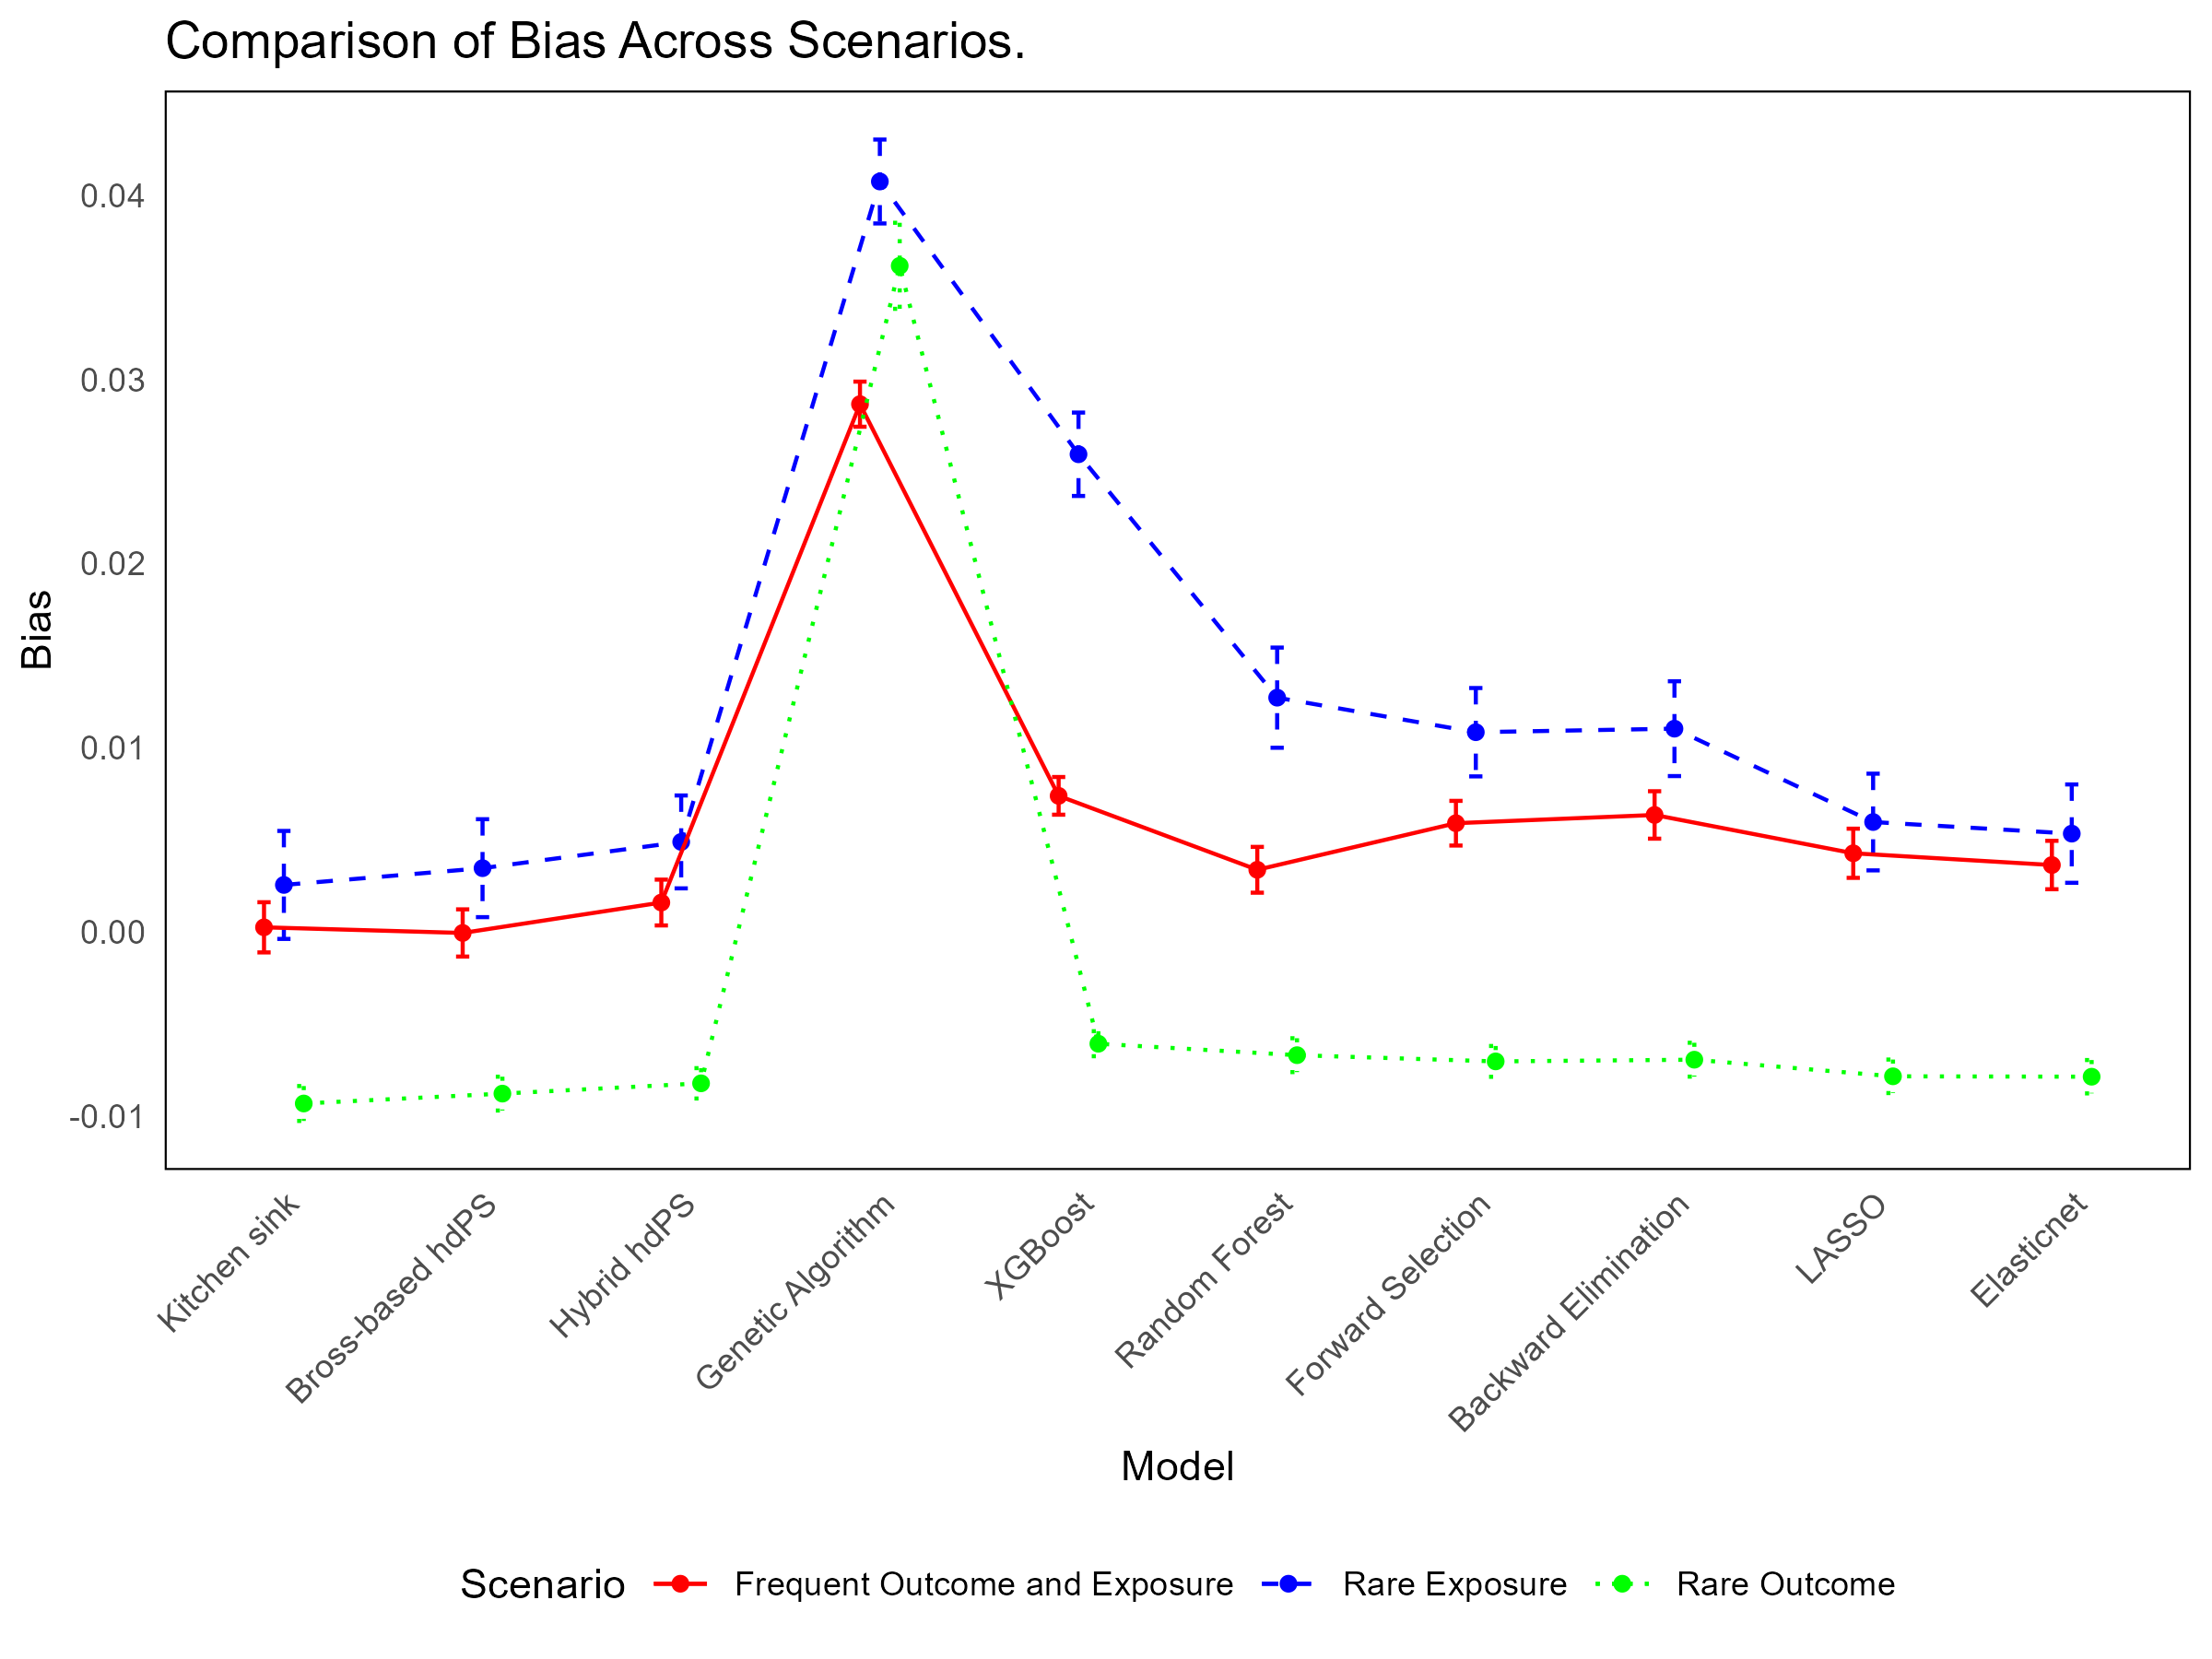
\includegraphics[width=1\linewidth,]{figures/metric_comparison_Bias} 

}

\caption{Comparison of Bias Across Different Methods in hdPS Analysis\label{fig:bias-comparison}}\label{fig:unnamed-chunk-1}
\end{figure}

\begin{figure}[th]

{\centering 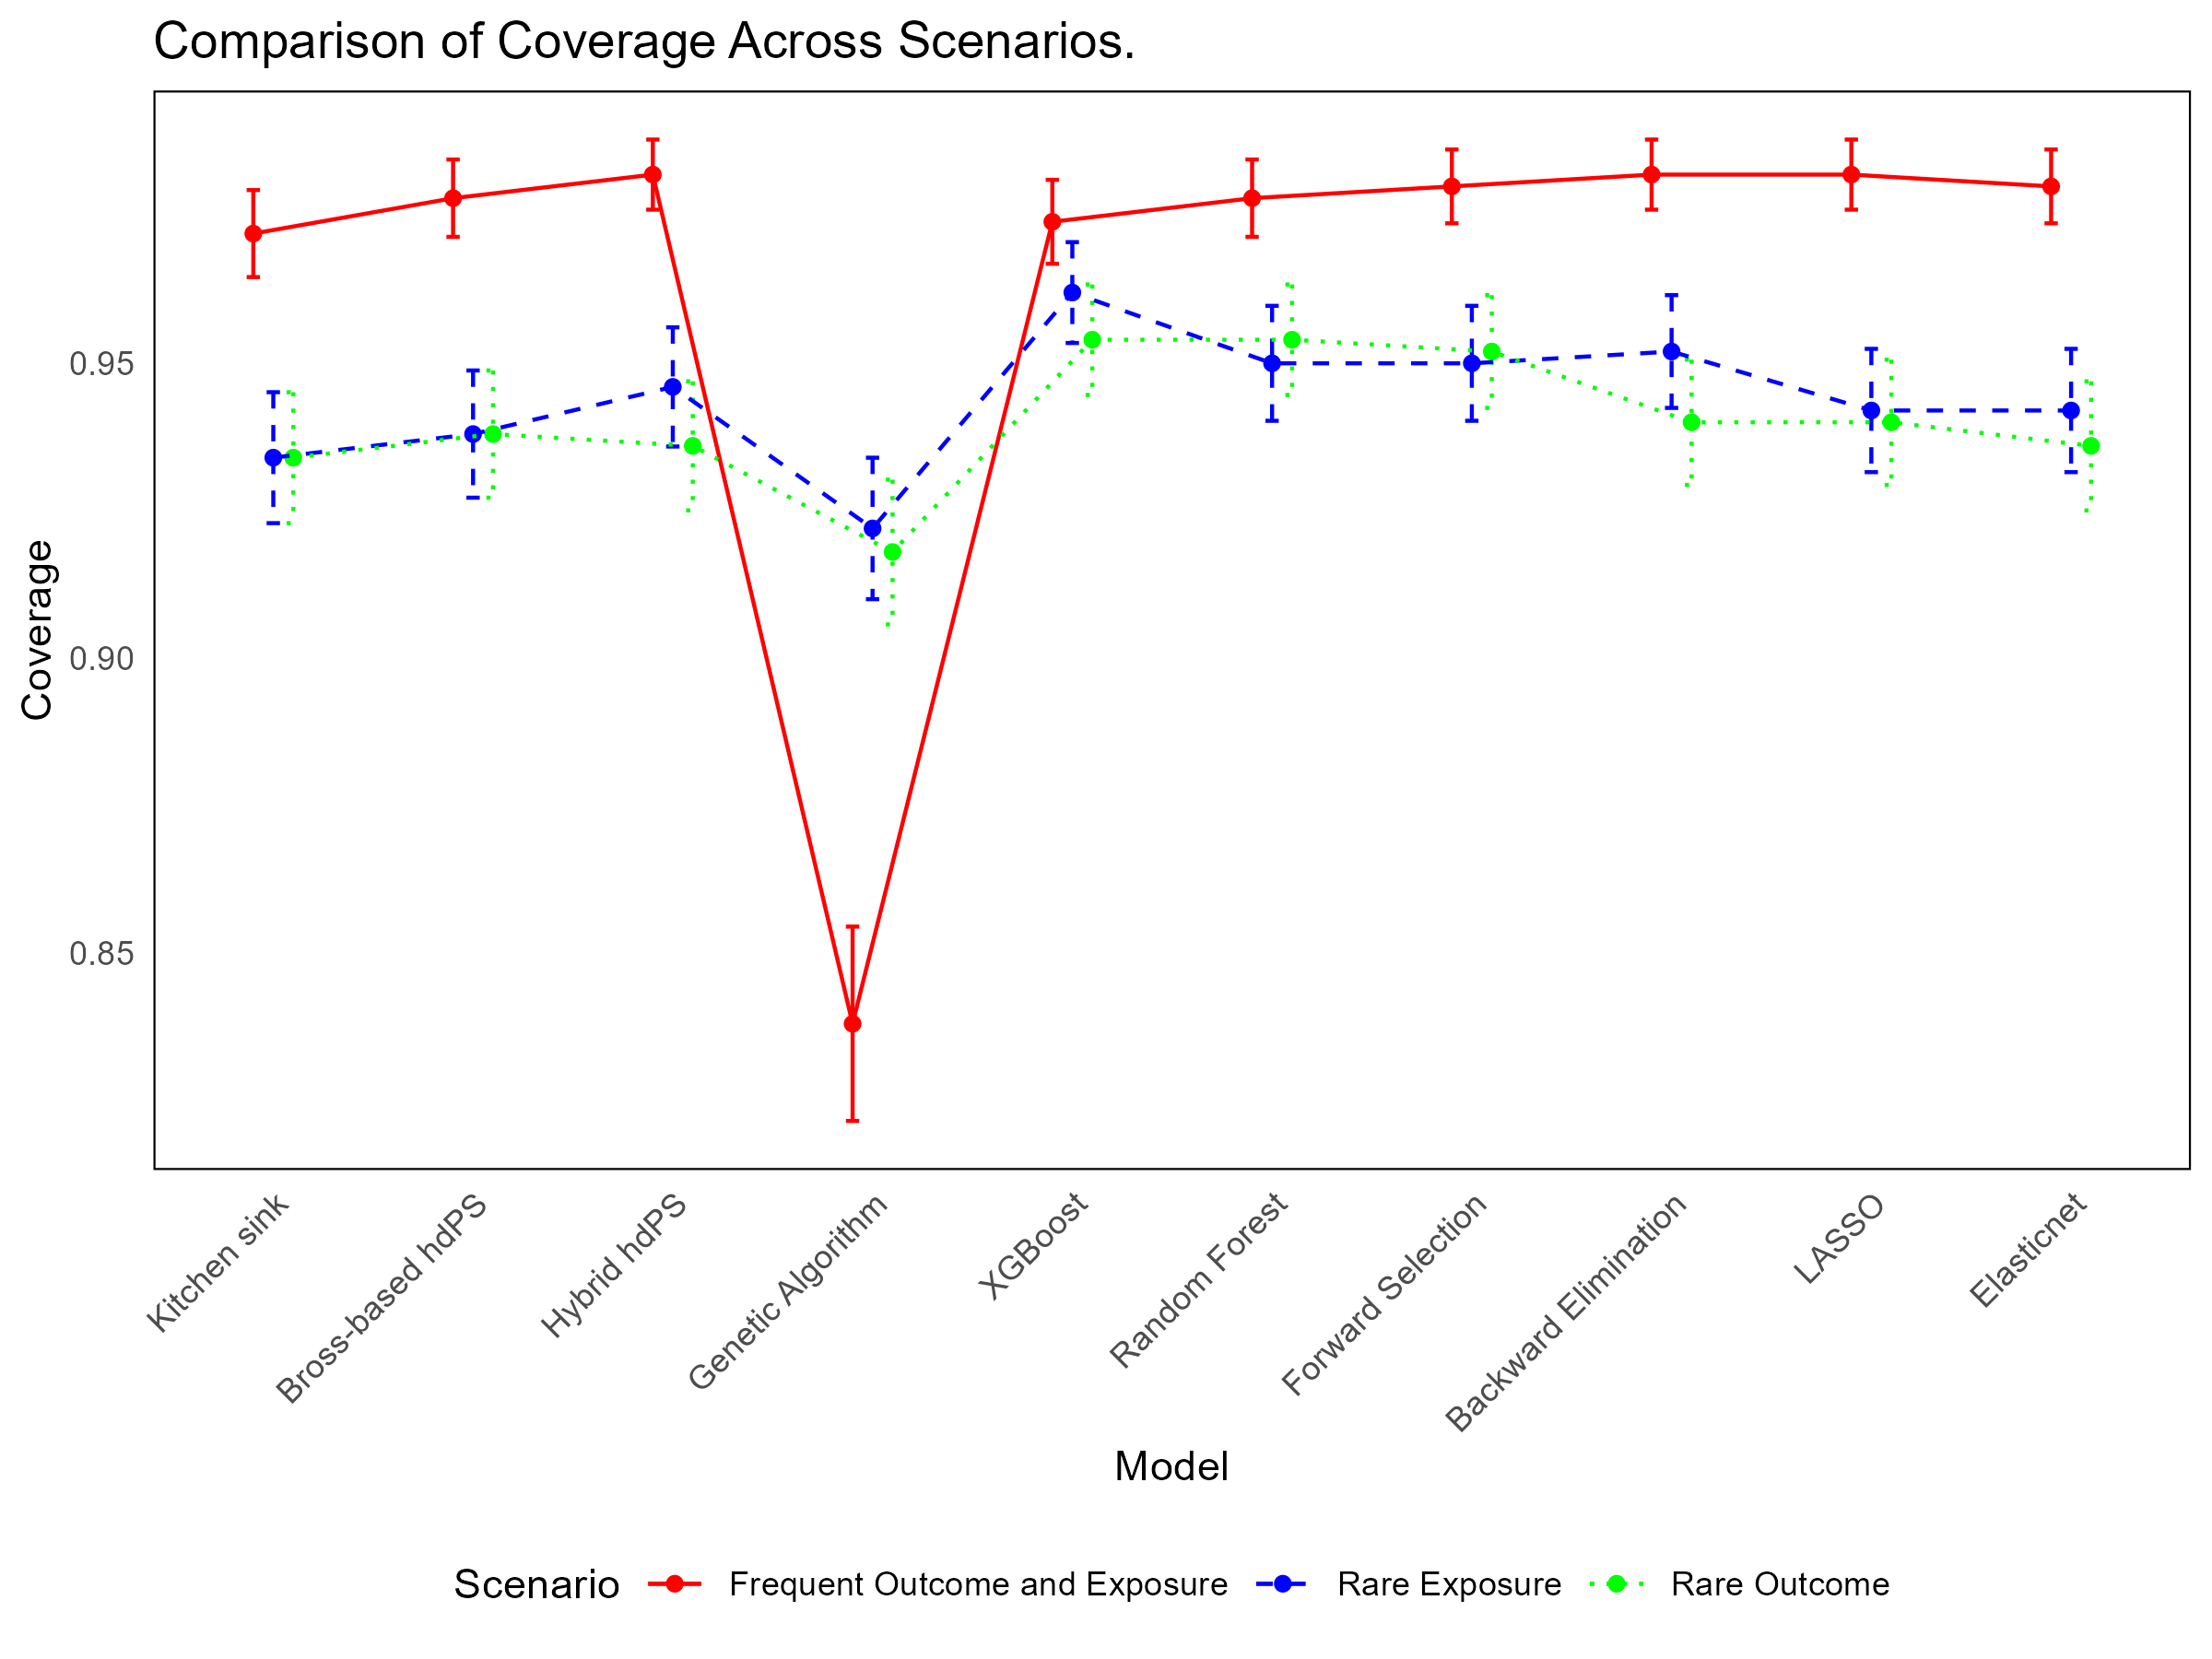
\includegraphics[width=1\linewidth,]{figures/metric_comparison_Coverage} 

}

\caption{Comparison of Coverage Probability Across Different Methods in hdPS Analysis\label{fig:Coverage-comparison}}\label{fig:unnamed-chunk-2}
\end{figure}

\section{Real-world analysis}\label{real-world-analysis}

\textcolor{red}{*Here we include full data analysis (with some summary results like exposure and outcome prevalence, and sample size) and report OR and RD. Also mention how many proxies were chosen (add in the picture of RD and OR; side by side for each method, ordered my magnitude of RD), and how many were in common with hdPS (add table).*}

See Figure \ref{fig:comparison-plot} for the results from analyzing the
NHANES (2013-2018) dataset.

\begin{figure}[th]

{\centering 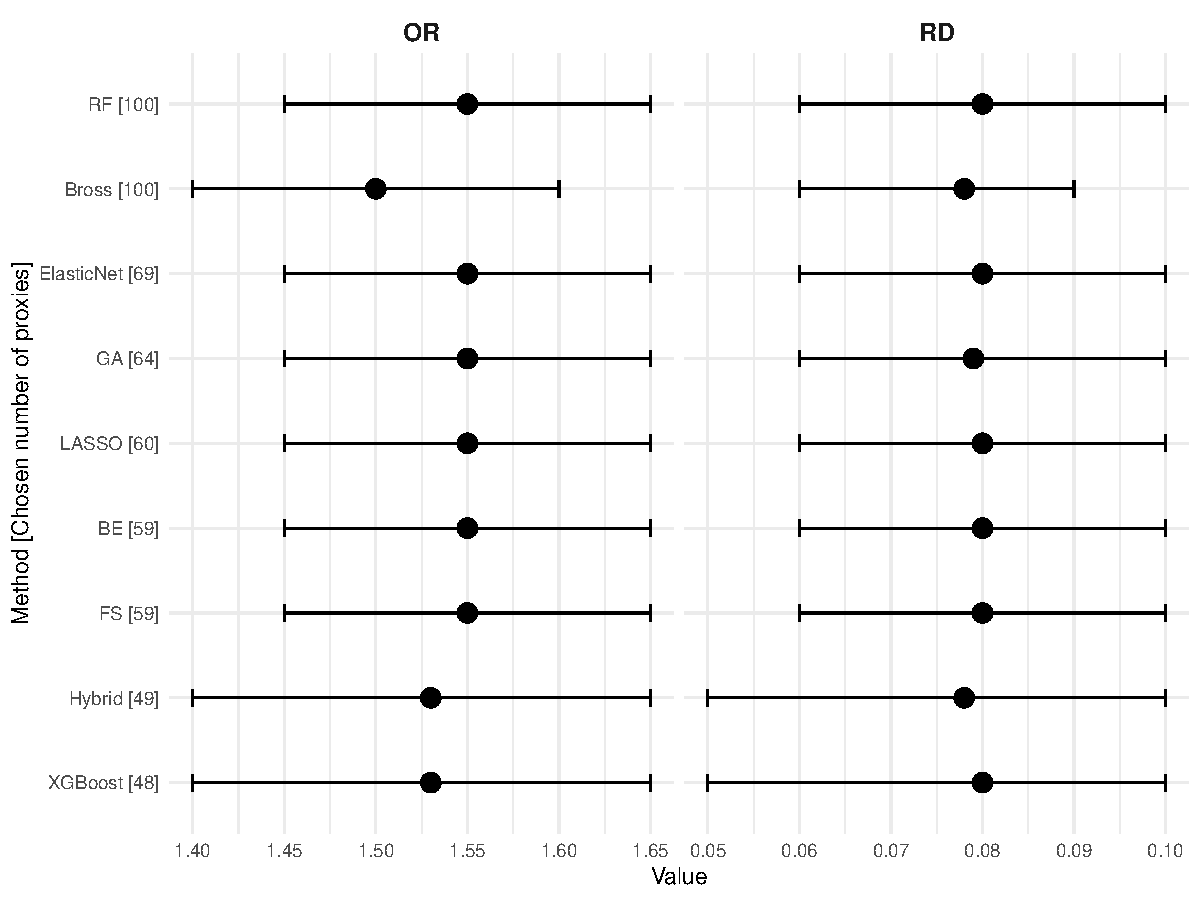
\includegraphics[width=1\linewidth,]{manuscript_files/figure-latex/unnamed-chunk-3-1} 

}

\caption{Figure presenting a comparison of Risk Differences (RD) and Odds Ratios (OR) with 95\% confidence intervals for different methods used to evaluate the association between obesity and diabetes risk. The analysis is based on data from the National Health and Nutrition Examination Survey (NHANES) for the years 2013-2018. Methods are arranged by the number of variables used in the models.\label{fig:comparison-plot}}\label{fig:unnamed-chunk-3}
\end{figure}

Table \ref{tab:method-comparison} presents a pairwise comparison of the
number of proxy features shared between different variable selection
methods used in the analysis. Each cell in the table indicates the count
of common proxy variables selected by the method in the corresponding
row and column. The diagonal cells, where the row and column methods are
the same, represent the total number of proxy variables selected
exclusively by each method.

\textcolor{red}{*need to think about how to best present this proxy in common table.*}

\begin{table}[htbp]
\centering
\caption{Comparison of variable overlap of selected proxies across different methods used to evaluate the association between obesity and diabetes}
\label{tab:method-comparison}
\begin{tabular}{lccccccccc}
\toprule
 & \textbf{Bross} & \textbf{Hybrid} & \textbf{LASSO} & \textbf{Elasticnet} & \textbf{GA} & \textbf{XGBoost} & \textbf{RF} & \textbf{FS} & \textbf{BE} \\
\midrule
\textbf{Bross formula} & 100 & & & & & & & & \\
\textbf{Hybrid (Bross and LASSO)} & 49 & 49 & & & & & & & \\
\textbf{LASSO} & 47 & 47 & 60 & & & & & & \\
\textbf{Elasticnet} & 54 & 48 & 60 & 69 & & & & & \\
\textbf{Genetic algorithm (GA)} & 44 & 28 & 36 & 40 & 64 & & & & \\
\textbf{XGBoost} & 38 & 24 & 28 & 30 & 25 & 48 & & & \\
\textbf{Random Forest (RF)} & 72 & 37 & 42 & 50 & 36 & 48 & 100 & & \\
\textbf{Forward selection (FS)} & 45 & 41 & 51 & 54 & 35 & 25 & 43 & 59 & \\
\textbf{Backward elimination (BE)} & 45 & 41 & 51 & 54 & 35 & 25 & 43 & 59 & 59 \\
\bottomrule
\end{tabular}
\end{table}

\textbf{Computing time}:

\textcolor{red}{*Report computing time for the Real-world analysis for each method. (add ordered table or figure)*}

\section{Discussion}\label{discussion}

\subsection{Summary of the simulation
findings}\label{summary-of-the-simulation-findings}

\textbf{Comparison of methods}:

Across the three scenarios---Frequent Exposure and Outcome, Rare
Exposure and Frequent Outcome, and Frequent Exposure and Rare
Outcome---XGBoost consistently exhibited the lowest Mean Squared Error
(MSE) and high coverage, making it one of the most reliable methods
overall. However, XGBoost did not always have the lowest bias; in fact,
methods such as the kitchen sink model, Bross-based hdPS, and Hybrid
hdPS often showed lower bias. The GA, in contrast, consistently
exhibited the highest bias and MSE, along with lower coverage and
greater variability, indicating it was less reliable for accurate effect
estimation. The kitchen sink model, while demonstrating low bias and
reasonable MSE, generally had higher variability and lower precision
compared to other methods like XGBoost. Methods such as Bross-based
hdPS, Hybrid hdPS, and Elasticnet performed moderately well across all
scenarios, balancing bias, coverage, and MSE, but they did not
outperform XGBoost in overall accuracy and precision.

\textbf{Comparison of scenarios}:

Scenarios with rare exposure tended to produce higher bias, particularly
for methods like GA and XGBoost, while frequent outcomes generally led
to lower bias. Overcoverage was common in the frequent exposure and
outcome scenario, while the other scenarios tended to have more balanced
or slightly under-coverage. Frequent exposure scenarios had higher
relative error, indicating more difficulty in precisely estimating
effects compared to rare exposure scenarios, which had lower relative
error. Rare outcome scenarios tended to have the lowest MSE, indicating
more precise effect estimates under these conditions, whereas rare
exposure scenarios had higher MSE, reflecting the challenges of
estimating effects when exposure is uncommon.

\subsection{Contextualizing the
literature}\label{contextualizing-the-literature}

\textcolor{red}{*need to write what hdps offers in the literature; what additional selection criteria was used so far*}

\subsection{Data analysis findings}\label{data-analysis-findings}

\textcolor{red}{*summarize real data analysis finding in 1 para*}

\subsection{Future Direction}\label{future-direction}

\textcolor{red}{*TMLE*}

\subsection{Conclusion}\label{conclusion}

In conclusion, this analysis highlights the importance of carefully
selecting appropriate methods for hdPS analysis based on the specific
characteristics of the data, particularly the prevalence of exposure and
outcome. While XGBoost consistently demonstrated strong performance in
terms of MSE and coverage, it did not always have the lowest bias,
suggesting that it may be most suitable when precision is prioritized
over bias minimization. GA, despite its potential, showed significant
limitations with consistently high bias and MSE, making it less reliable
for accurate effect estimation. The kitchen sink model, Bross-based
hdPS, and Hybrid hdPS methods provided a balanced approach, often
delivering low bias and moderate MSE, but with variability in coverage
depending on the scenario. Scenario-specific trends revealed that rare
outcomes generally yielded lower MSE and better precision, while rare
exposures were associated with higher bias and MSE, emphasizing the
challenges of accurately estimating effects in such contexts.
Ultimately, the findings underscore the need to tailor method selection
to the epidemiological scenario at hand, ensuring that the chosen
approach aligns with the specific goals and challenges of the analysis.

\section*{List of abbreviations}\label{list-of-abbreviations}
\addcontentsline{toc}{section}{List of abbreviations}

\begin{itemize}
\tightlist
\item
  hdPS: High-dimensional Propensity Score
\item
  NHANES: National Health and Nutrition Examination Survey
\item
  OR: Odds Ratio
\item
  RD: Risk Difference
\item
  SE: Standard Error
\item
  MSE: Mean Squared Error
\item
  LASSO: Least Absolute Shrinkage and Selection Operator
\item
  GA: Genetic Algorithm
\item
  RF: Random Forest
\item
  XGBoost: Extreme Gradient Boosting
\item
  FS: Forward Selection
\item
  BE: Backward Elimination
\item
  CV: Cross-Validation
\item
  RR: Relative Risk
\item
  Elasticnet: A regularized regression method that combines LASSO and
  Ridge regression
\end{itemize}

\section*{Declarations}\label{declarations}
\addcontentsline{toc}{section}{Declarations}

\subsection*{Ethics approval and consent to
participate}\label{ethics-approval-and-consent-to-participate}
\addcontentsline{toc}{subsection}{Ethics approval and consent to
participate}

The analysis conducted on secondary and de-identified data is exempt
from research ethics approval requirements. Ethics for this study was
covered by item 7.10.3 in University of British Columbia's Policy \#89:
Research and Other Studies Involving Human Subjects 19 and Article 2.2
in of the Tri-Council Policy Statement: Ethical Conduct for Research
Involving Humans (TCPS2).

\subsection*{Consent for publication}\label{consent-for-publication}
\addcontentsline{toc}{subsection}{Consent for publication}

\subsection*{Availability of data and
materials}\label{availability-of-data-and-materials}
\addcontentsline{toc}{subsection}{Availability of data and materials}

\subsection*{Competing interests}\label{competing-interests}
\addcontentsline{toc}{subsection}{Competing interests}

Over the past three years, MEK has received consulting fees from Biogen
Inc.~for consulting unrelated to this current work. MEK was previously
supported by the Michael Smith Foundation for Health Research Scholar
award.

\subsection*{Funding}\label{funding}
\addcontentsline{toc}{subsection}{Funding}

This work was supported by MEK's Natural Sciences and Engineering
Research Council of Canada (NSERC) Discovery Grants and Discovery
Accelerator Supplements.

\subsection*{Authors' contributions}\label{authors-contributions}
\addcontentsline{toc}{subsection}{Authors' contributions}

MEK: Conceptualization, Writing -- Original Draft, Review \& Editing YL:
Formal Analysis, Review \& Editing

\subsection*{Acknowledgements}\label{acknowledgements}
\addcontentsline{toc}{subsection}{Acknowledgements}

Not applicable.

\renewcommand\refname{References}
\bibliography{mergedbibliography.bib}


\end{document}
